%%===========================================================%%
%%                                                           %%
%%                        CORRECTIONS                        %%
%%                                                           %%
%%===========================================================%%


\chapter{Corrections}\label{chap:corrections}

\section{Method of corrections application}
\begin{equation}
  \frac{d\sigma}{dq} = \frac{1}{\Delta q} \times \frac{1}{\varepsilon} \times \frac{N^{\mathit{w}}-N^{\mathit{w}}_\textrm{bkgd}}{\mathit{L}_{\textrm{int}}^{\textrm{eff}}}
\end{equation}

%remembed about accounting for RP trigger eff!!!
\begin{equation}\label{eq:effectiveLumi}
	\mathit{L}_{\textrm{int}}^{\textrm{eff}} = \sum\limits_{\textrm{run}}\mathit{L}_{\textrm{int}}^{\textrm{run}} \times \epsilon_{\textrm{veto}}(L^{\textrm{run}})
\end{equation}
% \left(\epsilon_{\textrm{veto}}^{\textrm{online}} \oplus \epsilon_{\textrm{veto}}^{\textrm{offline}}(L_{\textrm{run}}) \right)

\begin{equation}
	\varepsilon = \epsilon_{\textrm{\tiny ET/IT}} \times \epsilon_{\textrm{vrtx}}(q) \times \epsilon_{\ref{enum:CutZVx}} \times \epsilon_{\ref{enum:CutDeltaZVx}} \times \epsilon_{\ref{enum:CutMissingPt}} \times \epsilon_{\textrm{\tiny PID}}(q)
\end{equation}

\begin{equation}
	N^{\mathit{w}} = \sum\limits_{\textrm{event}}\mathit{w}_{\textrm{event}}
\end{equation}



\begin{equation}
	\mathit{w} = \left[\prod\limits_{\textrm{sign}} \epsilon_{\textrm{\tiny TOF}}(\textrm{sign}, \textrm{PID}, p_{T},z_{vx},\eta)  \times \prod\limits_{\textrm{sign}} \epsilon_{\textrm{\tiny TPC}}(\textrm{sign}, \textrm{PID}, p_{T},z_{vx},\eta) \times \prod\limits_{\textrm{side}}\epsilon_{\textrm{\tiny RP}}^{\textrm{side}}(p_{x},p_{y}) \right]^{-1},
\end{equation}
\[\textrm{sign}\in\{+,-\},~~\textrm{side}\in\{E,W\}\]
% ()




\section{Efficiencies and acceptances}

In this section we present calculation of all efficiencies except TPC track reconstruction and TOF hit reconstruction and matching efficiency, which were discussed and presented in Ref.~\cite{supplementaryNote}.

\subsection{Trigger efficiency}\label{sec:triggerEff}
\subsubsection{Online veto (BBC-small and ZDC veto)}
%---------------------------
\begin{figure}[ht!]
\centering%
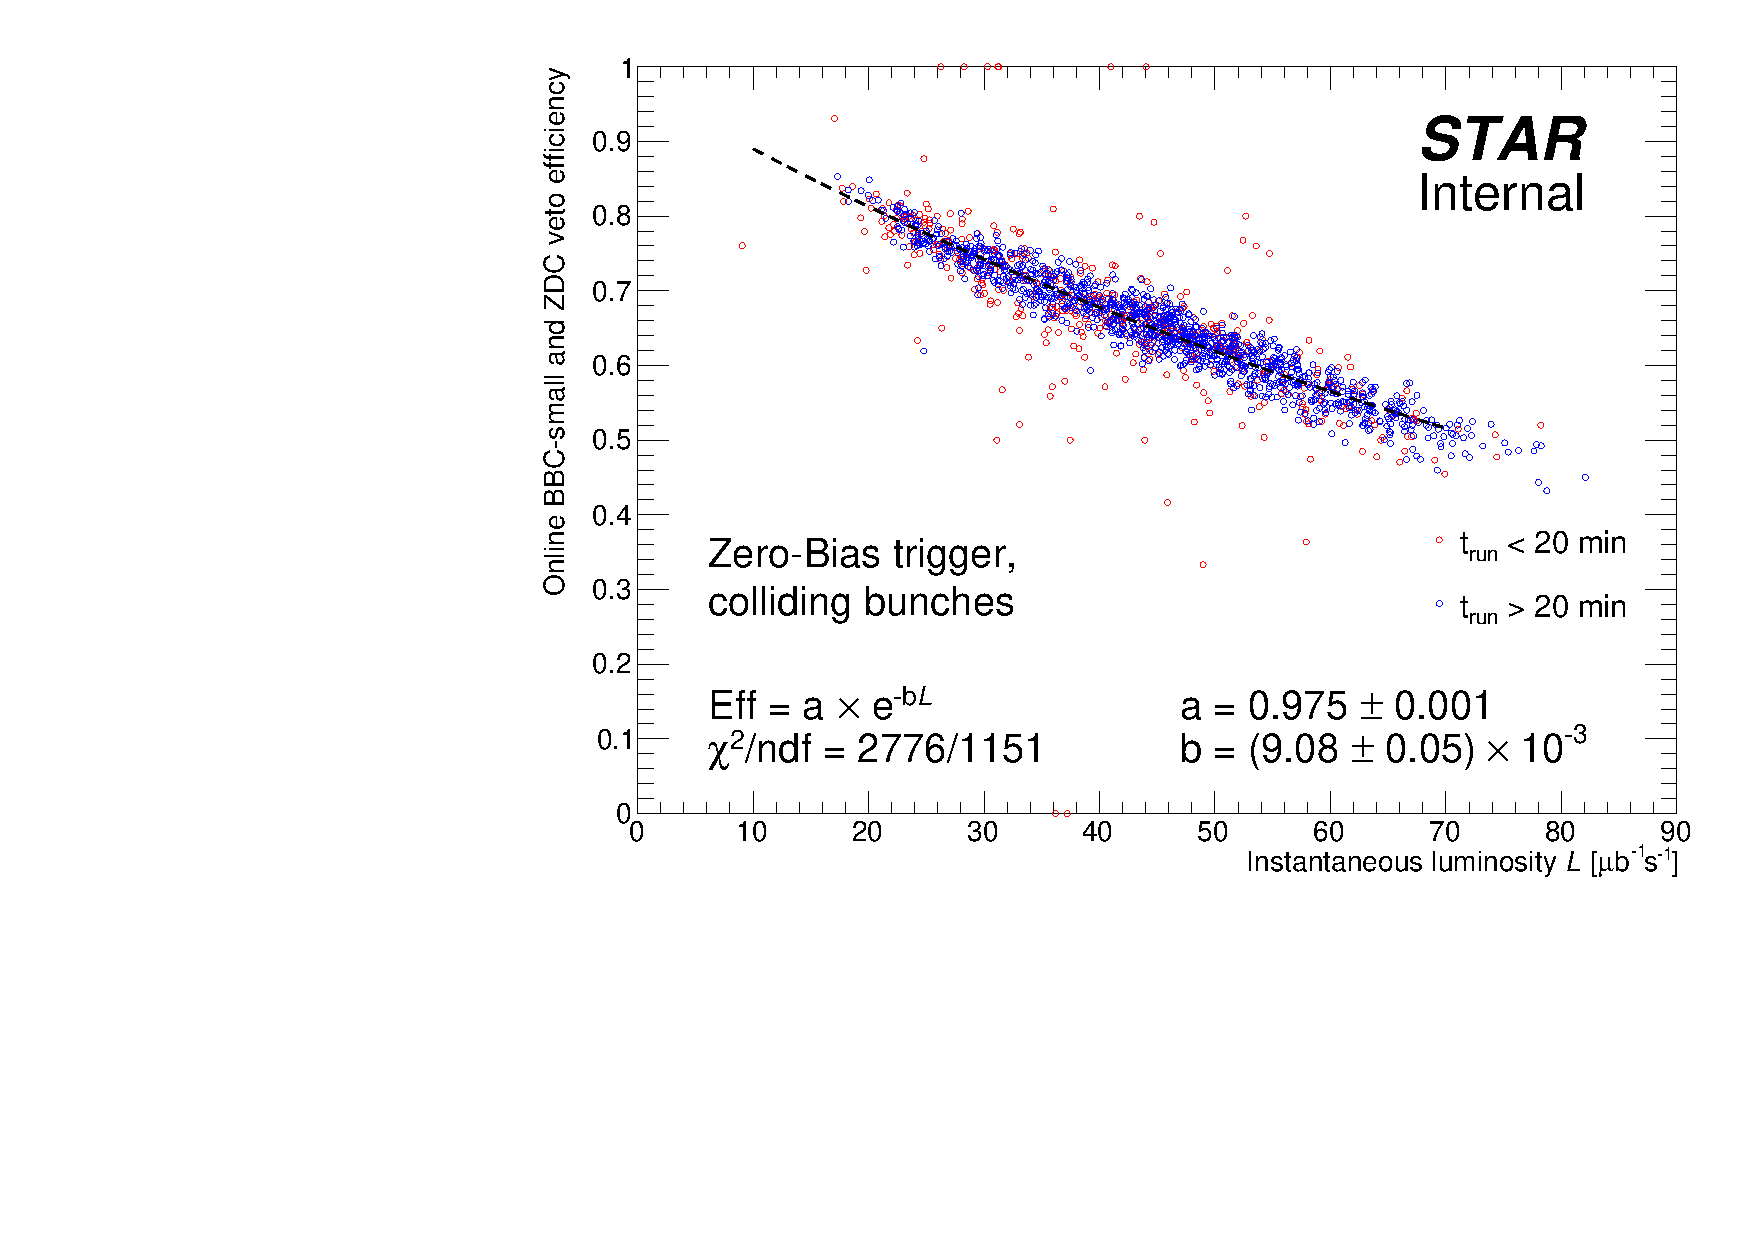
\includegraphics[width=0.65\linewidth,page=1]{graphics/corrections/OnlineVetoEffVsInstLumi_graph.pdf}%
\caption{Overall efficiency of the online BBC-small and ZDC veto as a function of instantaneous luminosity.}\label{fig:onlineVetoEff}%
\end{figure}
%---------------------------
\subsubsection{RP triggering efficiency}
\subsubsection{Up and Down RP combination veto}


\textbf{Oznaczenia:}\\[4pt]$\RPE$ - zrekonstruowany dokladnie jeden dobry slad po stronie EAST\\
$\RPW$ - zrekonstruowany dokladnie jeden dobry slad po stronie WEST\\
$\TRE$ - tryger w galezi z dobrym sladem po stronie EAST\\
$\TRNE$ - tryger w galezi bez dobrego sladu po stronie EAST\\
$\TRW$ - tryger w galezi z dobrym sladem po stronie WEST\\
$\TRNW$ - tryger w galezi bez dobrego sladu po stronie WEST\\
$\Vpu$ - weto trygera na jednoczesna kombinacje gora-dol spodowane przez pile-up\\
$\Vdm$ - weto trygera na jednoczesna kombinacje gora-dol spodowane przez oddzialywanie z materialem detektora\\
$\V$ - weto trygera na jednoczesna kombinacje gora-dol\\[20pt]\noindent%
%
Do tej pory sprawdzilem poprawke na wydajnosc rekonstrukcji sladow w Roman Potach po obu stronach:
\begin{equation}
\mbox{\LARGE$\varepsilon$}\left(\RPE\land\RPW\left|\TRE\land\TRW\right.\right) = 
\frac{\mbox{\LARGE$\varepsilon$}\left(\RPE\left|\TRE\right.\right) \times \mbox{\LARGE$\varepsilon$}\left(\RPW\left|\TRW\right.\right)}{1-\mbox{\LARGE$\varepsilon$}\left(!\RPE\land~!\RPW\Big|\TRE\land\TRW\Big.\right)}
\end{equation}  
Aby poprawic na calkowita wydajnosc przyadku zwiazana z trygerem i rekonstrukcja sladow w Roman Potach trzeba policzyc:
\begin{equation}
\mbox{\LARGE$\varepsilon$}\left(\RPE\land\RPW\land\TRE\land\TRW\land~!\V\right) = \mbox{\LARGE$\varepsilon$}\left(\RPE\land\RPW\left|\TRE\land\TRW\land~!\V\right.\right)\times\mbox{\LARGE$\varepsilon$}\left(\TRE\land\TRW\land~!\V\right)
\end{equation}
W przypadku czesci zwiazanej z wydajnoscia rekonstrukcji wystarczy zmodyfikowac dotychczas obliczone wydajnosci dodajac weta na jednoczesne kombinacje gora-dol w trygerze:
\begin{equation}
\mbox{\LARGE$\varepsilon$}\left(\RPE\land\RPW\left|\TRE\land\TRW\land~!\V\right.\right)=\frac{\mbox{\LARGE$\varepsilon$}\left(\RPE\left|\TRE\land~!\TRNE\right.\right) \times \mbox{\LARGE$\varepsilon$}\left(\RPW\left|\TRW\land~!\TRNW\right.\right)}{1-\mbox{\LARGE$\varepsilon$}\left(!\RPE\land~!\RPW\Big|\TRE\land\TRW\land~!\V\Big.\right)}
\end{equation}
Jesli chodzi o wydajnosc trygera to mysle, że trzeba oddzielic sama szanse detekcji protonow w Roman Potach w ktorych protony zostawiaja slad, oraz szanse na zawetowanie przypadku przez jednoczesny sygnal trygerowy gora-dol:
\begin{equation}
\mbox{\LARGE$\varepsilon$}\left(\TRE\land\TRW\land~!\V\right) = \mbox{\LARGE$\varepsilon$}\left(!\V\left|\TRE\land\TRW\right.\right)\times\mbox{\LARGE$\varepsilon$}\left(\TRE\land\TRW\right)
\end{equation}
Prawdopodobieństwo weta proponuje rozdzielic na dwie osobne komponenty - jedna zwiazana z pile-up'em, druga zwiazana z pojawieniem sie sygnalu w detektorze po drugiej stronie wiazki w wyniku interakcji protonu z materialem detektora:
\begin{equation}
\begin{split}
\mbox{\LARGE$\varepsilon$}\left(!\V\left|\TRE\land\TRW\right.\right)=\Bigg|\V=\Vpu\vee\Vdm\Bigg|=\\=1-\mbox{\LARGE$\varepsilon$}\left(\Vpu\left|\TRE\land\TRW\right.\right)-\mbox{\LARGE$\varepsilon$}\left(\Vdm\land~!\Vpu\left|\TRE\land\TRW\right.\right)
\end{split}
\end{equation}
Wydajnosc zwiazana z materialem martwym bede liczyl tak samo jak wydajnosc rekonstrukcji - w funkcji $z_{\text{vtx}}$, $p_{x}$ oraz $p_{y}$, natomiast wydajnosc zwiazana z pile-up'em chyba trzeba potraktowac jako jedna liczbe (osobna dla 4 kombinacji galezi) ktora policze osobno dla każdego runu a nastepnie dopasuje funkcje okreslajaca zależnosc tej poprawki od chwilowego lumi (dokladnie tak jak to robie z poprawka na weto na BBC, ZDC i slady w TPC/TOF).\\
Trzeba tutaj uważac żeby nie poprawiac weta przez pile-up dwukrotnie, tzn. może byc jednoczesne weto trygera w BBC-small i w RP spowodowane jakims przypadkiem dyfrakcyjnym (np. pojedyncza dyfrakcja, dyfrakcyjna dysocjacja). Mysle, że najlepiej bedzie policzyc laczna poprawke na weto w RP, BBC itd. z danych zerobias (wlaczyc RP do dotychczasowej poprawki na weto BBC + ...).\\
Wydajnosc samego trygerowania
\begin{equation}
\mbox{\LARGE$\varepsilon$}\left(\TRE\land\TRW\right) = \mbox{\LARGE$\varepsilon$}\left(\TRE\right) \times \mbox{\LARGE$\varepsilon$}\left(\TRW\right),
\end{equation}
\begin{equation}
\mbox{\LARGE$\varepsilon$}\left(\TRE\right) = \mbox{\LARGE$\varepsilon$}\left(\TRE_{1}\vee\TRE_{2}\right),~~~~\mbox{\LARGE$\varepsilon$}\left(\TRW\right) = \mbox{\LARGE$\varepsilon$}\left(\TRW_{1}\vee\TRW_{2}\right),
\end{equation}
dobrze bedzie policzyc już z danych, najlepiej elastycznych (ale można też z CD) patrzac jak czesto stacje z dobrymi sladami maja sygnal trygerowy.

\begin{equation}\begin{split}
\mbox{\LARGE$\varepsilon$}\left(\TRW\right) = \mbox{\LARGE$\varepsilon$}\left(\TRW\left|\RPE\&\RPW\&~!\TRNE\&~!\TRNW\right.\right) = \mbox{\LARGE$\varepsilon$}\left(\TRW_{1}\vee\TRW_{2}\left|\RPE\&\RPW\&~!\TRNE\&~!\TRNW\right.\right)=\\
=\mbox{\LARGE$\varepsilon$}\left(\TRW_{1}\left|\RPE\&\RPW\&~!\TRNE\&~!\TRNW\right.\right)+\mbox{\LARGE$\varepsilon$}\left(\TRW_{2}\left|\RPE\&\RPW\&~!\TRNE\&~!\TRNW\right.\right)+\\-\mbox{\LARGE$\varepsilon$}\left(\TRW_{1}\land\TRW_{2}\left|\RPE\&\RPW\&~!\TRNE\&~!\TRNW\right.\right)~~~~~\text{(analogicznie po stronie EAST)}
\end{split}\end{equation}


\subsection{Cuts efficiency}\label{sec:cutsEff}
\subsubsection{TPC \texorpdfstring{$z$}{z}-vertex cut~(\ref{enum:CutZVx})}
\subsubsection{TPC-RP \texorpdfstring{$z$}{z}-vertex matching~(\ref{enum:CutDeltaZVx})}
\subsubsection{Primary vertices limit~(\ref{enum:CutPrimVx}), BBC-large veto~(\ref{enum:CutBbcLarge}) and TOF clusters limit~(\ref{enum:CutTofClusters})}
%---------------------------
\begin{figure}[ht!]
\centering%
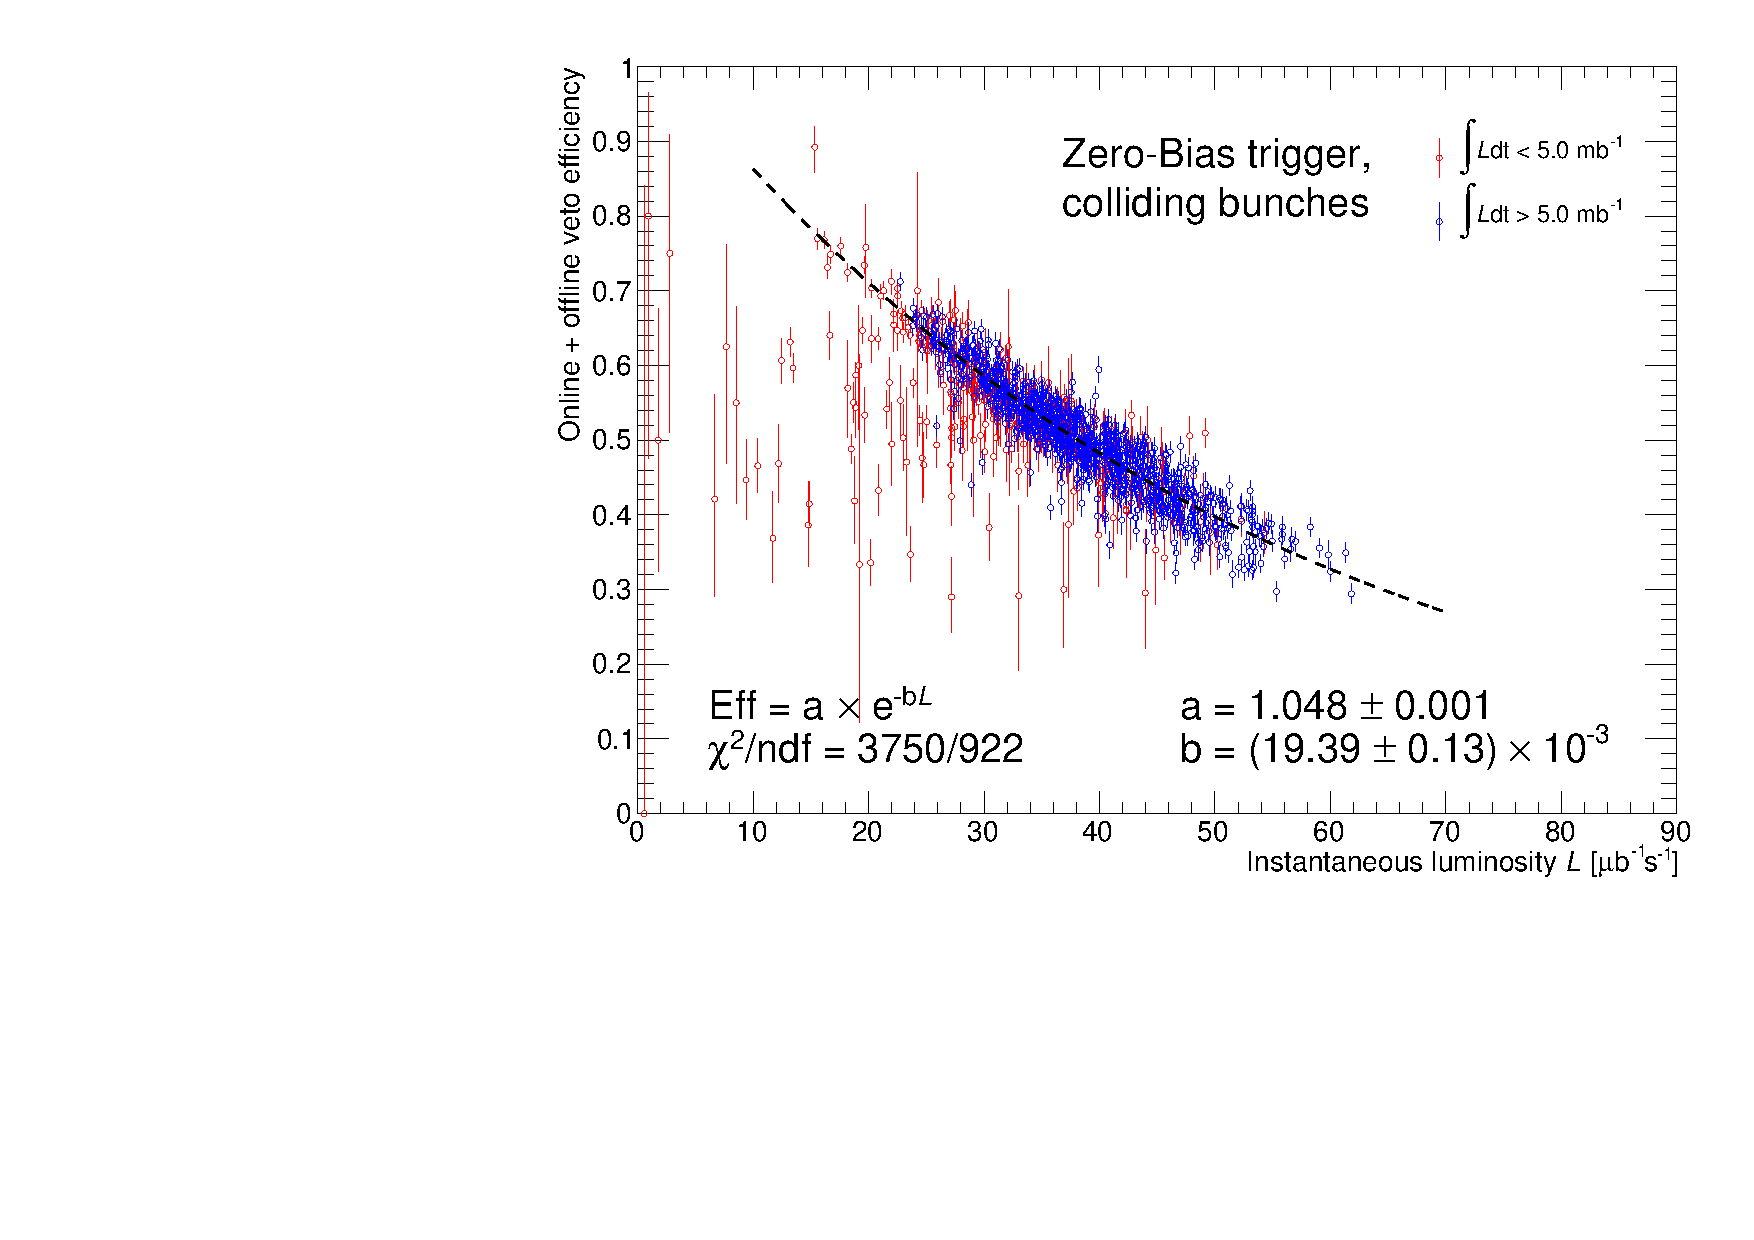
\includegraphics[width=0.65\linewidth,page=1]{graphics/corrections/OnlineAndOfflineVetoEffVsInstLumi_graph.pdf}%
\caption{Overall efficiency of the online BBC-small and ZDC veto, primary vertices limit~(\ref{enum:CutPrimVx}), BBC-large veto~(\ref{enum:CutBbcLarge}) and TOF clusters limit~(\ref{enum:CutTofClusters}) as a function of instantaneous luminosity.}\label{fig:onlineAndOfflineVetoEff}%
\end{figure}
%---------------------------
\subsubsection{Missing \texorpdfstring{$p_{T}$}{pT} cut~(\ref{enum:CutMissingPt})}
\subsubsection{Particle identification~(\ref{enum:CutPid})}


%---------------------------
\begin{figure}[ht!]
\centering
\parbox{0.315\textwidth}{
  \centering
  \begin{subfigure}[b]{\linewidth}{
                \subcaptionbox{\label{fig:sqMassTof_DataVsMC_pion}}{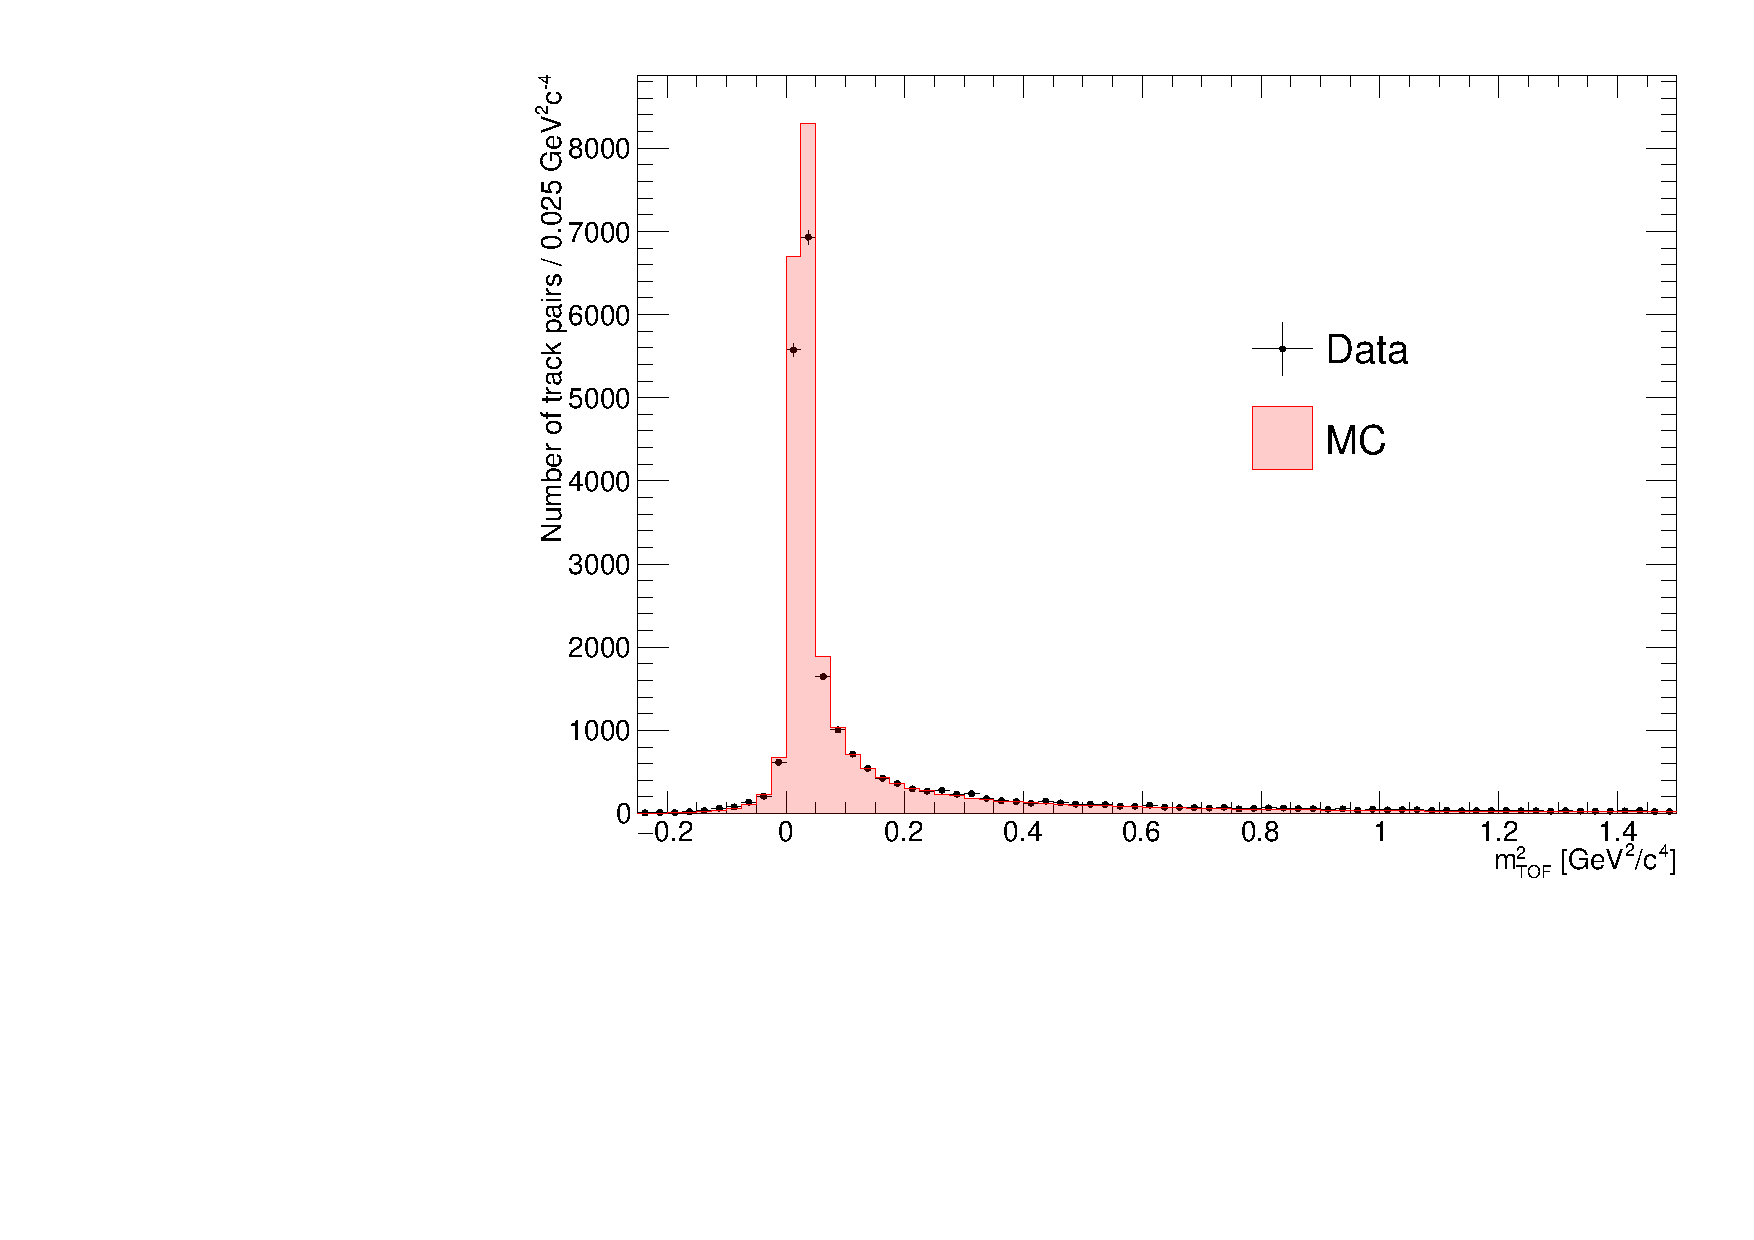
\includegraphics[width=\linewidth,page=1]{graphics/corrections/sqMassTof_DataVsMC.pdf}}}
  \end{subfigure}
}
\quad
\parbox{0.315\textwidth}{
  \centering
  \begin{subfigure}[b]{\linewidth}{
                \subcaptionbox{\label{fig:sqMassTof_DataVsMC_kaon}}{\includegraphics[width=\linewidth,page=2]{graphics/corrections/sqMassTof_DataVsMC.pdf}}}
  \end{subfigure}
}
\quad
\parbox{0.315\textwidth}{
  \centering
  \begin{subfigure}[b]{\linewidth}{
                \subcaptionbox{\label{fig:sqMassTof_DataVsMC_proton}}{\includegraphics[width=\linewidth,page=3]{graphics/corrections/sqMassTof_DataVsMC.pdf}}}
  \end{subfigure}
}%
\caption{Comparison of $m^{2}$ from TOF between data and MC for exclusive $\pi^{+}\pi^{-}$, $K^{+}K^{-}$ and $p\bar{p}$.}
\end{figure}
%---------------------------









\subsection{RP track acceptance and reconstruction efficiency}\label{sec:rpAccAndEff}

\subsection{TPC vertex reconstruction efficiency}\label{sec:tpcVxRecoEff}

The definition of vertex reconstruction efficiency established in this analysis is the probability that two global tracks, both associated with true-level primary particles from the kinematic region of the measurement, both satisfying kinematic and quality criteria (cuts~\ref{enum:TpcKinematicCuts} and ~\ref{enum:TpcQualityCuts}) and both matched with hits in TOF, form a vertex listed in the collection of reconstructed primary vertices and DCA(R) and DCA(z) of both global tracks calculated w.r.t. this vertex is contained within the limits of cut~\ref{enum:TpcDcaCuts}.

\section{Particle energy loss}\label{sec:energyLoss}
\section{Background subtraction}\label{sec:bkgdSubtraction}
\section{Unfolding}\label{sec:unfolding}

% 
%   W analizie CEP wydajnosc werteksowania to prawdopodobieństwo że
%  oba pierwotne slady z punktu B tworza werteks (to znaczy sa na liscie
%  sladow primary wspolnego werteksu i spelniaja ciecia DCA).
%  Nie patrzymy na dodatkowe werteksy, hity w TOF, BBC_small
% 
% E) --- pozostale wydajnosci
% 
%   w przypadku analizy CEP jest to pile-up czyli dodatkowy werteks lub
%   dodatkowy hit w TOF lub sygnal w BBC. Te poprawk mamy z embeddingu
%   patrzac ile przypadkow z D ma dodatkowy werteks, hist w TOF lub BBC
% 
%   To samo powinnismy dostac z analizy "naszych" zero-bias.
% 
%   W przypadku analizy SD mamy pile-up czyli dodatkowy werteks, BBC
%   po stronie protonu też to znamy z embeddingu lub "naszych" zero-bias.
% 
%   Dodatkowo dochodza dodatkowe werteksy z oddzialywań wtornych/rozpadow.
%   Ten efekt znamy z MC. Powinno byc to samo z pile-up'em jak i  bez
% 
% 
% Jakies uwagi?
